\documentclass[a4paper,10pt]{article}
\usepackage[utf8]{inputenc}
\usepackage[english]{babel}
\usepackage{indentfirst}
\usepackage{geometry}
\usepackage{fancyhdr} % For custom headers
\usepackage{lastpage} % To determine the last page for the footer
\usepackage{extramarks} % For headers and footers
\usepackage[most]{tcolorbox} % For problem answer sections
\usepackage{graphicx,subfigure} % For inserting images
\usepackage{color,soul} % For link coloring
\usepackage[hidelinks]{hyperref} % For URL links (no box or color name)
\usepackage{csquotes}
\usepackage[labelfont=bf]{caption}
\usepackage{textcomp}
\usepackage{enumitem}
\usepackage{fourier}
\usepackage{listings}


\definecolor{mygreen}{RGB}{28,172,0} % color values Red, Green, Blue
\definecolor{mylilas}{RGB}{170,55,241}


% Margins
\geometry{
a4paper,
tmargin=1in,
bmargin=1in,
lmargin=1in,
rmargin=1in,
textwidth=6.5in,
textheight=9.0in,
headsep=0.25in
}

% Header and footer
\pagestyle{fancy}
\lhead{SCERPA documentation} % Top left header
\chead{} % Top center header
\rhead{VLSI Lab\firstxmark} % Top right header
\lfoot{\myDueDate} % Bottom left footer
\cfoot{} % Bottom center footer
\rfoot{Page\ \thepage\ of\ \pageref{LastPage}} % Bottom right footer
\renewcommand\headrulewidth{0.4pt} % Size of the header rule
\renewcommand\footrulewidth{0.4pt} % Size of the footer rule

% Other configurations
\setlength\parindent{0pt} % Removes all indentation from paragraphs
\setlength\parskip{1pt} % Ensures paragraphs are still recognizable as such
%\setcounter{secnumdepth}{0} % Removes default section numbers
\setcounter{tocdepth}{3} % Sets depth of table of contents
\linespread{1.1}

% Template values
\newcommand{\myFirstLogo}{vlsilogo.png}
\newcommand{\mySecondLogo}{polito_logo.png}
\newcommand{\myName}{Giuliana Beretta}
\newcommand{\myEmail}{giuliana.beretta@polito.it}
\newcommand{\myColleagueName}{Yuri Ardesi}
\newcommand{\myColleagueEmail}{yuri.ardesi@polito.it}
\newcommand{\myTitle}{SCERPA documentation}
\newcommand{\VLSItitle}{VLSI Lab - Politecnico di Torino}
\newcommand{\VLSIdep}{Department of Electronics and Telecommunications}
\newcommand{\VLSIurl}{https://www.vlsilab.polito.it/}
\newcommand{\authorTitle}{Authors}
\newcommand{\myDueDate}{June 2020}

%----------------------------------------------------------------------------------------
%  DOCUMENT STRUCTURE (MACROS & ENVIRONMENTS)
%----------------------------------------------------------------------------------------

% Colored links macro
%\newcommand{\hrefcol}[3] {\href{#1}{\textcolor{#3}{#2}}}
\setlength\parindent{24pt}

% Macro for custom title page signature header
\newsavebox{\myLogos}
\sbox{\myLogos}{%
\begin{tabular*}{\textwidth}{@{}l@{}r@{\extracolsep{0.125in}}l@{}}%
\parbox{9cm}{\raggedright{\includegraphics[width=4.5cm]{\myFirstLogo}}} &
\parbox{9cm}{\raggedright{\includegraphics[width=6cm]{\mySecondLogo}}}
\end{tabular*}}


\begin{document}
%\lstset{language=Matlab,%
%    %basicstyle=\color{red},
%    breaklines=true,%
%    morekeywords={matlab2tikz},
%    keywordstyle=\color{blue},%
%    morekeywords=[2]{1}, keywordstyle=[2]{\color{black}},
%    identifierstyle=\color{black},%
%    stringstyle=\color{mylilas},
%    commentstyle=\color{mygreen},%
%    showstringspaces=false,%without this there will be a symbol in the places where there is a space
%    numbers=left,%
%    numberstyle={\tiny \color{black}},% size of the numbers
%    numbersep=9pt, % this defines how far the numbers are from the text
%    emph=[1]{for,end,break},emphstyle=[1]\color{red}, %some words to emphasise
%    %emph=[2]{word1,word2}, emphstyle=[2]{style},    
%}
\lstloadlanguages{Matlab}%
\lstset{language=Matlab,                        % Use MATLAB
        frame=single,                           % Single frame around code
        basicstyle=\small\ttfamily,             % Use small true type font
        keywordstyle=[1]\color{blue}\bfseries,        % MATLAB functions bold and blue
        keywordstyle=[2]\color{mylilas},         % MATLAB function arguments purple
        keywordstyle=[3]\color{blue}\underbar,  % User functions underlined and blue
        identifierstyle=,                       % Nothing special about identifiers
                                                % Comments small dark green courier
        commentstyle=\usefont{T1}{pcr}{m}{sl}\color{mygreen}\small,
        stringstyle=\color{mylilas},             % Strings are purple
        showstringspaces=false,                 % Don't put marks in string spaces
        tabsize=5,                              % 5 spaces per tab
        %
        %%% Put standard MATLAB functions not included in the default
        %%% language here
        morekeywords={xlim,ylim,var,alpha,factorial,poissrnd,normpdf,normcdf},
        %
        %%% Put MATLAB function parameters here
        morekeywords=[2]{on, off, interp},
        %
        %%% Put user defined functions here
        morekeywords=[3]{FindESS, homework_example},
        %
        morecomment=[l][\color{blue}]{...},     % Line continuation (...) like blue comment
        numbers=left,                           % Line numbers on left
        firstnumber=1,                          % Line numbers start with line 1
        numberstyle=\tiny\color{blue},          % Line numbers are blue
        stepnumber=5                            % Line numbers go in steps of 5
        }

% Blank out the traditional title page
\title{\vspace{-1in}} % no title name
\author{} % no author name
\date{} % no date listed
\maketitle % makes this a title page

% Use custom title macro instead
\usebox{\myLogos}
\vspace{0.3in} % spacing below title header

% Assignment title
\begin{center}
	\begin{minipage}{\textwidth}
		\begin{flushleft}
			\textbf{\VLSItitle} \hfill \textbf{\authorTitle}\\
			\VLSIdep \hfill \myColleagueName~~-~~\myColleagueEmail\\
			\VLSIurl \hfill \myName~-~\myEmail\\
		\end{flushleft}
	\end{minipage}
\end{center}
{\centering \noindent\rule{\textwidth}{0.4pt} \par}


\vspace{1.3cm}
{\centering \Huge \textbf{\textsc{\myTitle}} \par}
\vspace{1.3cm}
{\centering \noindent\rule{\textwidth}{0.4pt} \par}
\vspace{1.3cm}

% Table of Contents
%\tableofcontents
%\newpage
\section{Introduction}
\noindent In this file are explained the mandatory and optional fields for the input script of SCERPA. 
In the input script MUST be present the \textit{circuit} definition, and there is the possibility to specify the \textit{settings}.

\section{Circuit definition}
\noindent There are \underline{two} possibilities to describe the circuit layout:
\begin{enumerate}
\item using MagCAD\footnote{https://topolinano.polito.it/the-project/} and extracting the \textit{.qll} file;
\item using MATLAB and specifying the structure's fields described below.
\end{enumerate}

\noindent For the second case, there are some fields which are mandatory, and are identified by the symbol \danger . The reference system is shown in \figurename~\ref{fig:ref_sys}.

\begin{figure}[h!]
	\centering
	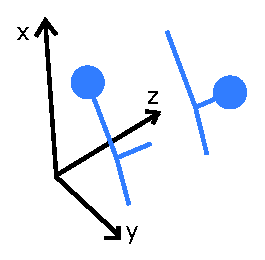
\includegraphics[scale=0.8]{axis.eps}
	\caption{Reference system for the circuit layout.}
	\label{fig:ref_sys}
\end{figure}

\begin{description}
\item[dist\_z] a value which specify the intermolecular distance along the z-axis in \r{A}ngstr\"{o}m [\textit{default} 10~\AA]
\item[dist\_y] a value which specify the intermolecular distance along the y-axis in \r{A}ngstr\"{o}m [\textit{default} 10.145~\AA~\footnote{The value corresponds to default \textbf{dist\_z} + inter-dot distance of the bisferrocene.}]
\item[molecule] a char vector containing the name of the molecules, chosen from the \underline{Molecule list} below, even those in brackets [\textit{default} bisfe\_4] 
\item[components] a matrix, with the same dimensions of the \textbf{structure}, containing in each position the molecule type expressed with the corresponding number in the \underline{Molecule list} below [\textit{default} all elements equal to \textbf{molecule}] \footnote{If \textbf{components} is present, the field \textbf{molecule} is not taken into account. If \textbf{components} is missing, the circuit is composed with the same molecule in each position, and the molecule used is the one specified in the \textbf{molecule} field (default or not).}
\item[structure \danger] a matrix which specify the circuit layout. In each position one can insert a driver or a molecule. Drivers are identified by the string \textit{Dr}, molecules are identified by the number of the clock zone to which they belong.   
\item[Values\_Dr \danger] a matrix in which for each driver (row) is specified its input voltage for each time step (column)
\item[stack\_phase \danger] a matrix in which for each clock zone (row) is specified the clock voltage for each time step (column).
\item[rotation\_x] a matrix, with the same dimensions of the \textbf{structure}, containing in each position the molecule rotation around the x-axis expressed in degree [\textit{default} 0\textdegree]
\item[rotation\_y] a matrix, with the same dimensions of the \textbf{structure}, containing in each position the molecule rotation around the y-axis expressed in degree [\textit{default} 0\textdegree]
\item[rotation\_z] a matrix, with the same dimensions of the \textbf{structure}, containing in each position the molecule rotation around the z-axis expressed in degree [\textit{default} 0\textdegree]
\item[shift\_x] a matrix, with the same dimensions of the \textbf{structure}, containing in each position the molecule shift along the x-axis expressed in \r{A}ngstr\"{o}m [\textit{default} 0~\AA]
\item[shift\_y] a matrix, with the same dimensions of the \textbf{structure}, containing in each position the molecule shift along the y-axis expressed in \r{A}ngstr\"{o}m [\textit{default} 0~\AA]
\item[shift\_z] a matrix, with the same dimensions of the \textbf{structure}, containing in each position the molecule shift along the z-axis expressed in \r{A}ngstr\"{o}m [\textit{default} 0~\AA]
\item[Vext] a matrix, with the same dimensions of the \textbf{structure}, containing in each position the fixed external voltage applied onto the molecule expressed in volts [\textit{default} 0~V]
\end{description}



\subsection*{Molecules list}
\noindent Below the list of the available molecules with the identification number used in SCERPA. The terms in brackets specify which molecule is actually associated to the \textit{circuit.molecule} field. 
\begin{itemize}
\item[0 ] $\longrightarrow$  bisfe4\_ox\_counterionOnCarbazole
\item[1 ] $\longrightarrow$  bisfe4\_ox\_counterionOnThiol (bisfe\_4)
\item[2 ] $\longrightarrow$  bisfe4\_ox\_counterionOnThiol\_orca (bisfe\_4\_orca)
\item[3 ] $\longrightarrow$  bisfe4\_ox\_noCounterion
\item[4 ] $\longrightarrow$  bisfe4\_ox\_noCounterion\_TSA\_2states
\item[5 ] $\longrightarrow$  bisfe4\_ox\_noCounterion\_TSA\_3states
\item[6 ] $\longrightarrow$  bisfe4\_sym
\item[7 ] $\longrightarrow$  butane\_ox\_noCounterion (butane)
\item[8 ] $\longrightarrow$  butane\_ox\_noCounterion\_orca
\item[9 ] $\longrightarrow$  butaneCam
\item[10] $\longrightarrow$  decatriene\_ox\_noCounterion (decatriene)
\item[11] $\longrightarrow$  linear\_mol\_w7\_a2000 (linear\_w7)
\item[12] $\longrightarrow$  linear\_mol\_w7\_a3000
\item[13] $\longrightarrow$  linear\_mol\_w9\_a3000 (linear\_w9)
\item[14] $\longrightarrow$  linear\_mol\_w95\_a3000 (linear\_w95)
\end{itemize}


\section{SCERPA settings}
\noindent In the following are listed and explained the fields of the structure for the definition of the code settings.

\begin{description}
%\item[Time definition]: 
%	\begin{itemize}
%	\item \underline{timestep}: [\textit{default} 1]
%	\end{itemize}
\item[Topo integration]:
	\begin{itemize}
	\item \underline{magcadImporter}: set to 1 whether layout is designed with magCAD, 0 otherwise [\textit{default} 0]
	\item \underline{doubleMolDriverMode}: set to 1 whether the input drivers should be represented with two molecules, 0 otherwise [\textit{default} 0]
	\end{itemize}
\item[Energy]:
	\begin{itemize}
	\item \underline{energyEval}: set to 1 whether one wants to evaluate the internal energy, the exchange energy, the clock energy, and the total energy. Set to 0 otherwise [\textit{default} 0] \textcolor{red}{non funziona}
	\end{itemize}
\item[Output/Plot]:
	\begin{itemize}
	\item \underline{plot\_plotAbsoluteCharge}: if set to 1 it plots the absolute value of the dots charge in the 3D layout plot, otherwise it considers the actual value of the dots charge [\textit{default} 1] 
	\item \underline{plotIntermediateSteps}: \textcolor{red}{non esiste} [\textit{default} 0] 
	\item \underline{plotActiveRegionWindow}: \textcolor{red}{grafico da sistemare} [\textit{default} 0] 
	\item \underline{plot\_3dfig}: if set to 1 it plots the 3D layout of the circuit for each time step [\textit{default} 1] 
	\item \underline{plot\_voltage}: if set to 1 it plots the input voltage on each molecule for each time step [\textit{default} 1] 
	\item \underline{plot\_chargeFig}: if set to 1 it plots the charge value of the logic dots for each molecule, and for each time step [\textit{default} 1] 
	\item \underline{plot\_logic}: \textcolor{red}{dà errore} [\textit{default} 0] 
	\item \underline{plot\_clock}: \textcolor{red}{da sistemare} [\textit{default} 0]
	\item \underline{plot\_molnum}: if set to 1, it writes the molecule label in the 3D layout plot [\textit{default} 1] 
	\item \underline{verbosity}: this setting defines how much informations are written in the console during the simulation, if set to 0 means that no data are written, if set to 1 the convergence step is written for each time step, if set to 2 convergence info are written for each time step [\textit{default} 0] 
	\item \underline{pauseStep}: \textcolor{red}{non funziona} [\textit{default} 0] 
	\item \underline{fig\_saver}: \textcolor{red}{dà errore} [\textit{default} 'no'] 
	\end{itemize}
\item[Convergence settings]:
	\begin{itemize}
	\item \underline{max\_step}: set the maximum number of SCF iterations, after having reached this value, precision is lowered to LP and then to LLP if needed (see Precision settings below) [\textit{default} 1000] 
	\item \underline{immediateUpdate}: if set to 1, the algorithm updates the charge value onto the dots at each sub-step, one molecule at a time. This let the algorithm to converge faster, but it is far from the physical behaviour, since molecules actually \enquote{update} all together. To speed up the convergence without loosing the physical meaning, one should appropriately choose the damping factor. Hint: set this setting to 0, unless strictly needed [\textit{default} 1] 
	\item \underline{damping}: damping affects the rate and mode of convergence without influencing the final result, if correctly chosen. Value must be in range [0 - 1), hint: 0.2 [\textit{default} 0.0] 
	\end{itemize}
\item[Convergence accelerations]:
	\begin{itemize}
	\item \underline{enableRefining}: if set to 1, once the algorithm reaches convergence it disables the active region and continues the evaluation, it stops otherwise [\textit{default} 1] 
	\item \underline{enableActiveRegion}: if set to 1, the algorithm evaluates the interaction among a reduced set of molecule, otherwise it considers the whole set of molecules even if they are very far in the layout [\textit{default} 1] 
	\item \underline{activeRegionThreshold}: this value defines which molecules belong to the active region, if the voltage variation is higher  the this value, the molecule is added to the active region list [\textit{default} 0.0015] 
	\item \underline{enableInteractionRadiusMode}: \textcolor{red}{che differenza c'è con activeRegion?} [\textit{default} 1] 
	\item \underline{interactionRadius}: \textcolor{red}{come sopra} [\textit{default} 101] 
	\end{itemize}
\item[DEBUG informations]:
	\begin{itemize}
	\item \underline{printConvergenceTable}: \textcolor{red}{non c'è??} [\textit{default} 0] 
	\end{itemize}
\item[Precision]:
	\begin{itemize}
	\item \underline{LPmode}: maximum number of steps to try to reach convergence in Low Precision Mode [\textit{default} 200] 
	\item \underline{LPPmode}: maximum number of steps to try to reach convergence in Very Low Precision Mode [\textit{default} 300] 
	\item \underline{conv\_threshold\_HP}: when the SCF error reaches the convergence threshold, the algorithm stops. If it is not reached, precision is lowered to LP and and the algorithm runs in LPmode. If convergence is not achieved even in this mode, precision is lowered to LLP and and the algorithm runs in LLPmode [\textit{default} 0.000005] 
	\item \underline{conv\_threshold\_LP}: convergence threshold in Low Precision Mode [\textit{default} 0.0005] 
	\item \underline{conv\_threshold\_LLP}: convergence threshold in Very Low Precision Mode [\textit{default} 0.005] 
	\end{itemize}
\item[MATLAB optimization]:
	\begin{itemize}
	\item \underline{enableJit}: \textcolor{red}{non c'è??} [\textit{default 1}] 
	\end{itemize}
\item[Driver saturation]:
	\begin{itemize}
	\item \underline{driverSaturation}: set to 1 whether the charge values of the driver should saturate, 0 otherwise [\textit{default} 0]
	\end{itemize}
\end{description}


\section{Examples}
\subsection{MagCAD layout}
\lstinputlisting{magCAD_example.m}

\subsection{MATLAB layout}
\lstinputlisting{matlab_example.m}

\end{document}